\documentclass[11pt, a4paper, twocolumn]{article}

% Fonts and math (Elsevier-like Times style)
\usepackage{graphicx} % Required for inserting images
\usepackage{array} % For extra column formatting
\usepackage{amsmath, amssymb, cancel} % for equation environment
\usepackage{float,geometry}
\geometry{margin=2cm}
\usepackage[skip=10pt]{parskip}
\usepackage{setspace}
\usepackage{hyperref}
\usepackage{cite, bookmark}
\usepackage{url}
\usepackage[table,xcdraw]{xcolor}
\usepackage[export]{adjustbox}
\usepackage{listings,pdfpages}
\usepackage{dblfloatfix}

% --- Abstract styling (elsarticle look)
\usepackage{abstract}
\renewcommand{\abstractnamefont}{\normalfont\bfseries}
\renewcommand{\abstracttextfont}{\normalfont}
\renewenvironment{abstract}{%
  \par\noindent\rule{\linewidth}{0.4pt}\par
  \begin{center}\bfseries Abstract\end{center}%
}{%
  \par\rule{\linewidth}{0.4pt}\par
}

% --- Section styling (similar to elsarticle
\usepackage{titlesec}
\titleformat{\section}{\normalfont\large\bfseries}{\thesection.}{0.5em}{}
\titleformat{\subsection}{\normalfont\normalsize\bfseries}{\thesubsection.}{0.5em}{}

% Table of contents styling
\usepackage{tocloft}
\cftsetindents{section}{0em}{2em}
\cftsetindents{subsection}{1em}{2em}
\renewcommand\cfttoctitlefont{\hfill\Large\bfseries}
\renewcommand\cftaftertoctitle{\hfill\mbox{}}
\renewcommand\cftfigfont{\footnotesize}
\renewcommand\cftfigpagefont{\footnotesize}
\renewcommand\cftloftitlefont{\large}

\graphicspath{ {./images/} }

\definecolor{blurple}{HTML}{5865F2}
\definecolor{backcolour}{HTML}{272823}

\hypersetup{
    colorlinks=true,
    linkcolor=black,
    urlcolor=black,
    citecolor=blurple,
}

\urlstyle{same}

\DeclareMathOperator{\sinc}{sinc}

\renewcommand{\arraystretch}{1.4}

% Python code export
\lstset{
    language=Python,
    basicstyle=\ttfamily\scriptsize,
    keywordstyle=\color{teal},       
    commentstyle=\color{gray},        
    stringstyle=\color{magenta},  
    showstringspaces=false,
    frame=single,
    breaklines=true,
    numbers=left,
    numberstyle=\tiny\color{gray}
}

\setcounter{secnumdepth}{5}
\setcounter{tocdepth}{5}

%%%%%%%%%%%%%%%%%%%%%%%%%%%%%%%%%%%

\title{%


\includegraphics[width=0.2\linewidth]{ucd_brandmark_black.jpg} \vspace{0.5cm}\\

{\Large\bfseries UCD School of Physics}\vspace{1.5cm}\\

{\large PHYC30170 Physics Astronomy and Space Lab I}\\
{\bfseries CCD and Spectroscopy}

}
\author{Joana C.C. Adao \\ \small Student No.: 23311051}
\date{\today}

\begin{document}

% Title page - single column
\onecolumn
\maketitle

% Abstract - single column
\thispagestyle{empty}
\begin{abstract}

In this experiment, a charge-coupled device (CCD) camera was characterised by determining its gain and readnoise using bias and flat
field frames. The CCD was then used in a spectrograph configuration to capture spectral images of Mercury and Sodium lamps, allowing
for calibration and resolution determination of the spectrograph. The CCD average gain was found to be \textbf{0.2700 e$^-$/ADU} and
readnoise to be \textbf{4.4722 e$^-$}, consistent with manufacturer specifications. The spectrograph was calibrated using known
Mercury emission lines, yielding a calibration curve of $y = 0.2071 x + 333.646$, with an uncertainty of \textbf{0.7399 nm}. Attempts
to resolve the Sodium D-lines were limited by detector saturation and insufficient line separation. As a result, the spectrograph's
resolution was determined by fitting Gaussians to the well-defined Mercury lines, giving resolving powers of \textbf{R = 296.0 ± 11.3} at
436 nm and \textbf{R = 221.0 ± 12.0} at 546 nm. The results obtained demonstrated reliable CCD performance and effective spectrograph
calibration, though limitation in resolving closely spaced lines was noted.

\end{abstract}

\newpage

% Table of Contents - single column
\tableofcontents
\pagenumbering{roman}
\setcounter{page}{2}

\newpage

%%%%%%%%%%%%%%%%%%%%%%%%%%%%%%%%%%%

% Start main content in two columns
\twocolumn
\pagenumbering{arabic}
\setcounter{page}{1}

\section{Introduction} \label{sec:1}

\subsection{Charge-Coupled Devices (CCDs)}

Charge-coupled devices, or CCDs, are semiconductor devices primarily made of silicon that are used to detect and capture images through
the photoelectric effect by converting incoming photons (light) into electrical signals that are then stored in a potential well until they
are "read out" and processed by a computer to create digital images or into raw count data, which is particularly useful in scientific 
applications such as photometry. \cite{ccdsucd,bakich2023intro,Tulloch2005CCDs}

CCDs can be "frontside illuminated" or "backside illuminated". For frontside illuminated CCDs, the incoming light must pass through several
layers of the CCD structure before reaching the photosensitive area. This can lead to some loss of sensitivity, especially for shorter 
wavelengths of light, like blue or ultraviolet light. \cite{ccdsucd,bakich2023intro}

Backside illuminated CCDs have been "thinned" such that light strikes the photosensitive area directly, making it more sensitive to a 
larger range of wavelengths, including blue and ultraviolet light. However, if the detector is thinned too much the quantum efficiency,
which is the measure of how effectively a CCD converts incoming photons into electrons, can decrease as photons will not produce
electrons. For good blue quantum efficiency, the CCD should be thinned to about 15-20 microns, though signals near infrared
wavelengths may be lost. \cite{bakich2023intro,detectionoflight}

\begin{figure}[hb]
  \centering
  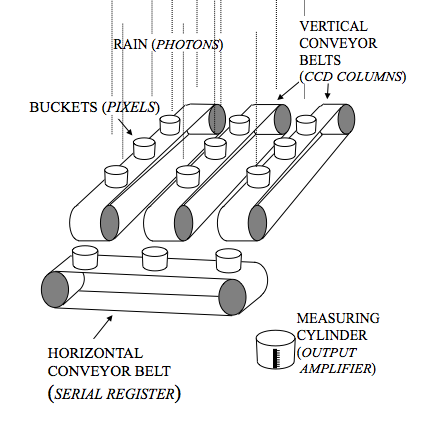
\includegraphics[width=.85\linewidth]{bucket_brigade.png}
  \caption{Illustration of the bucket brigade analogy for CCD operation. \protect{\cite{Tulloch2005CCDs}}}
  \label{fig:1}
\end{figure}

\subsubsection{CCD Operation}

For the understanding of CCD operation, an analogy to a bucket brigade is often used, Figure \ref{fig:1}.

In this analogy, each pixel in the CCD is represented as a bucket distributed across a field (CCD array) that collects water 
(electrons) when it rains (photons hitting the CCD). After the rainstorm (exposure), the buckets are passed along conveyor belts
(shifted) to a central collection metre (readout register) one row at a time. Once the buckets reach the collection metre, the 
amount of water in each bucket is measured (CCD readout or image) and recorded. \cite{ccdsucd,Tulloch2005CCDs,howell2000handbook}

\subsubsection{Darks, Flats, Biases}

As with any imaging system, CCDs are subject to various sources of noise and imperfections that can affect the quality of the captured images.
To reduce these effects, scientists often use calibration frames, which include dark, flat, and bias frames.

\textbf{Dark frames} are images taken with the shutter closed and with the same exposure time as the science images. They capture the thermal 
noise generated by the CCD's electronic components, known as 'dark current'. By subtracting the dark frame from the science image, this 
noise can be reduced. However, most modern CCDs are cooled to low temperatures using liquid nitrogen to minimise thermal noise, 
making dark frames less critical for clear images and data. \cite{bakich2023intro,Tulloch2005CCDs,ccdsucd}

\textbf{Flat fields} are images taken of an uniformly illuminated surface, such as a blank screen or the twilight sky. These images are used to correct
for variations in pixel sensitivity, vignetting, and other optical imperfections such as dust on the CCD chip or window. Several flat field
images are typically taken and averaged together to create a 'master' field, which is then divided across the science images to correct for
these variations. \cite{bakich2023intro,Tulloch2005CCDs,ccdsucd}

\textbf{Bias frames} are images, usually taken before the dark frames, with the shutter closed and with zero exposure time. They capture the electronic
offset of the CCD, and it represents the zero-point, or base-line signal level of the CCD. Any "hot" or defective pixels in the CCD will 
appear brightly, alongside any gradients caused by the readout electronics limitations. By subtracting the bias frame from the science image,
usually several are taken and averaged to create a 'master', the electronic offset can be corrected for. For n frames, the readnoise is 
reduced by a factor of $\sqrt{n}$. \cite{bakich2023intro,Tulloch2005CCDs,ccdsucd}

\subsection{Spectroscopy}

When light hits a wall or obstacle, like a diffraction grating, it bends around it and the wavelengths that make up the light spread out into a 
spectrum in a phenomenon called diffraction. Light of different wavelengths diffracts at different angles following \( n\lambda = d \sin \theta\), with
d as the distance between gaps, \(\lambda\) as the wavelength of light, n as the order of diffraction, and \(\theta\) as the angle of diffraction.
\cite{ccdsucd}

A \textbf{spectrograph} is an instrument that uses this principle to separate incoming light into its component wavelengths, allowing for detailed
analysis of the light's spectral properties. A classical configuration spectrograph will consist of a telescope, a slit, a collimator, a diffraction
grating, and a camera, as seen in Figure \ref{fig:2}. \cite{ccdsucd}

\begin{figure}[h]
  \centering
  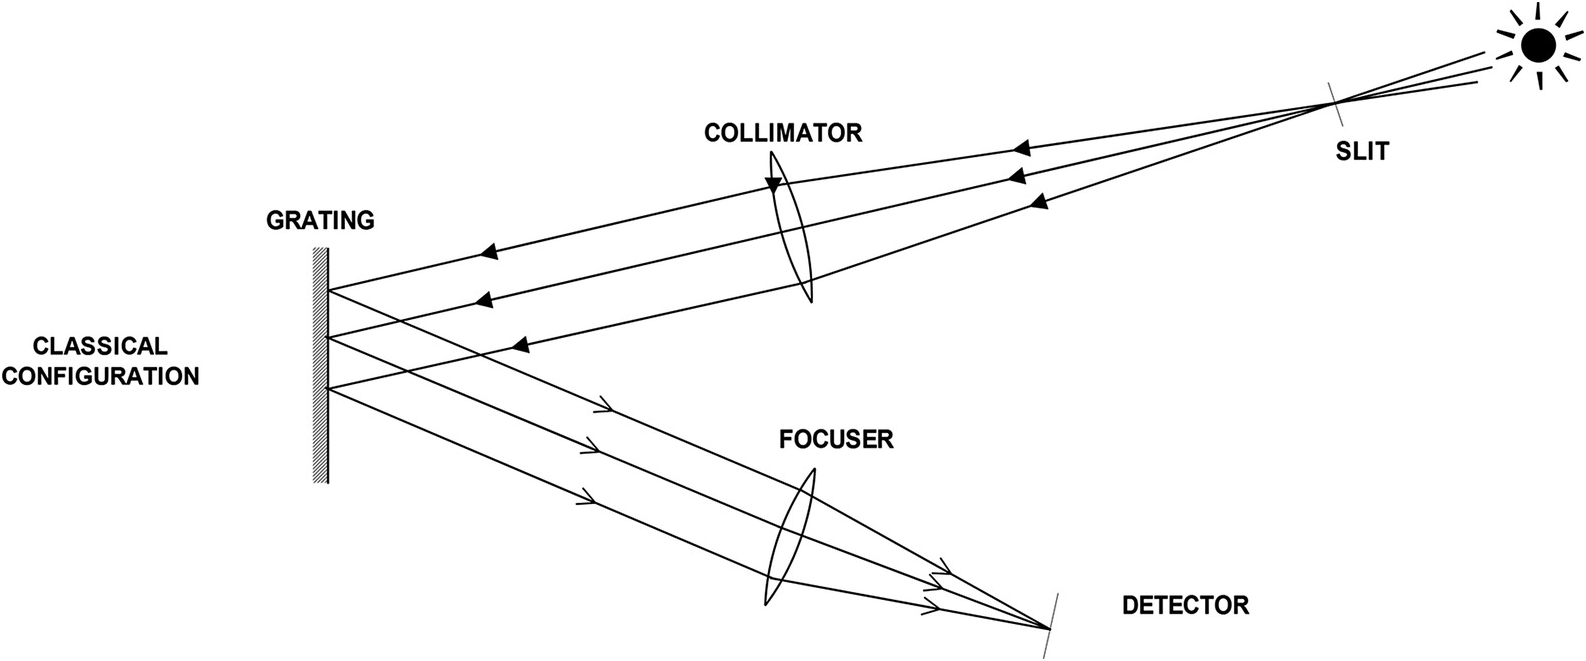
\includegraphics[width=.99\linewidth]{urn_cambridge.org_id_binary_20170717115824452-0433_9781316694435_16618fig5_1.png}
  \caption{Schematic diagram of a classical configuration spectrograph. \protect{\cite{Trypsteen_Walker_2017}}}
  \label{fig:2}
\end{figure}

The telescope collects and focuses the incoming light onto the slit, which cuts the light into a narrow beam or "slice". The collimator takes this
diverging beam of light and converts it into a parallel beam, which is then directed onto the diffraction grating. The grating is what determines the
spectral resolution of the spectrograph as it disperses the light into its component wavelengths. Finally, the camera captures the dispersed light
and records the resulting spectrum, often using a CCD detector for high sensitivity and resolution. \cite{ccdsucd}

\section{Methodology} \label{sec:2}

The experimental setup used in this lab is shown in Figure \ref{fig:3}. 

\begin{figure}[ht]
  \centering
  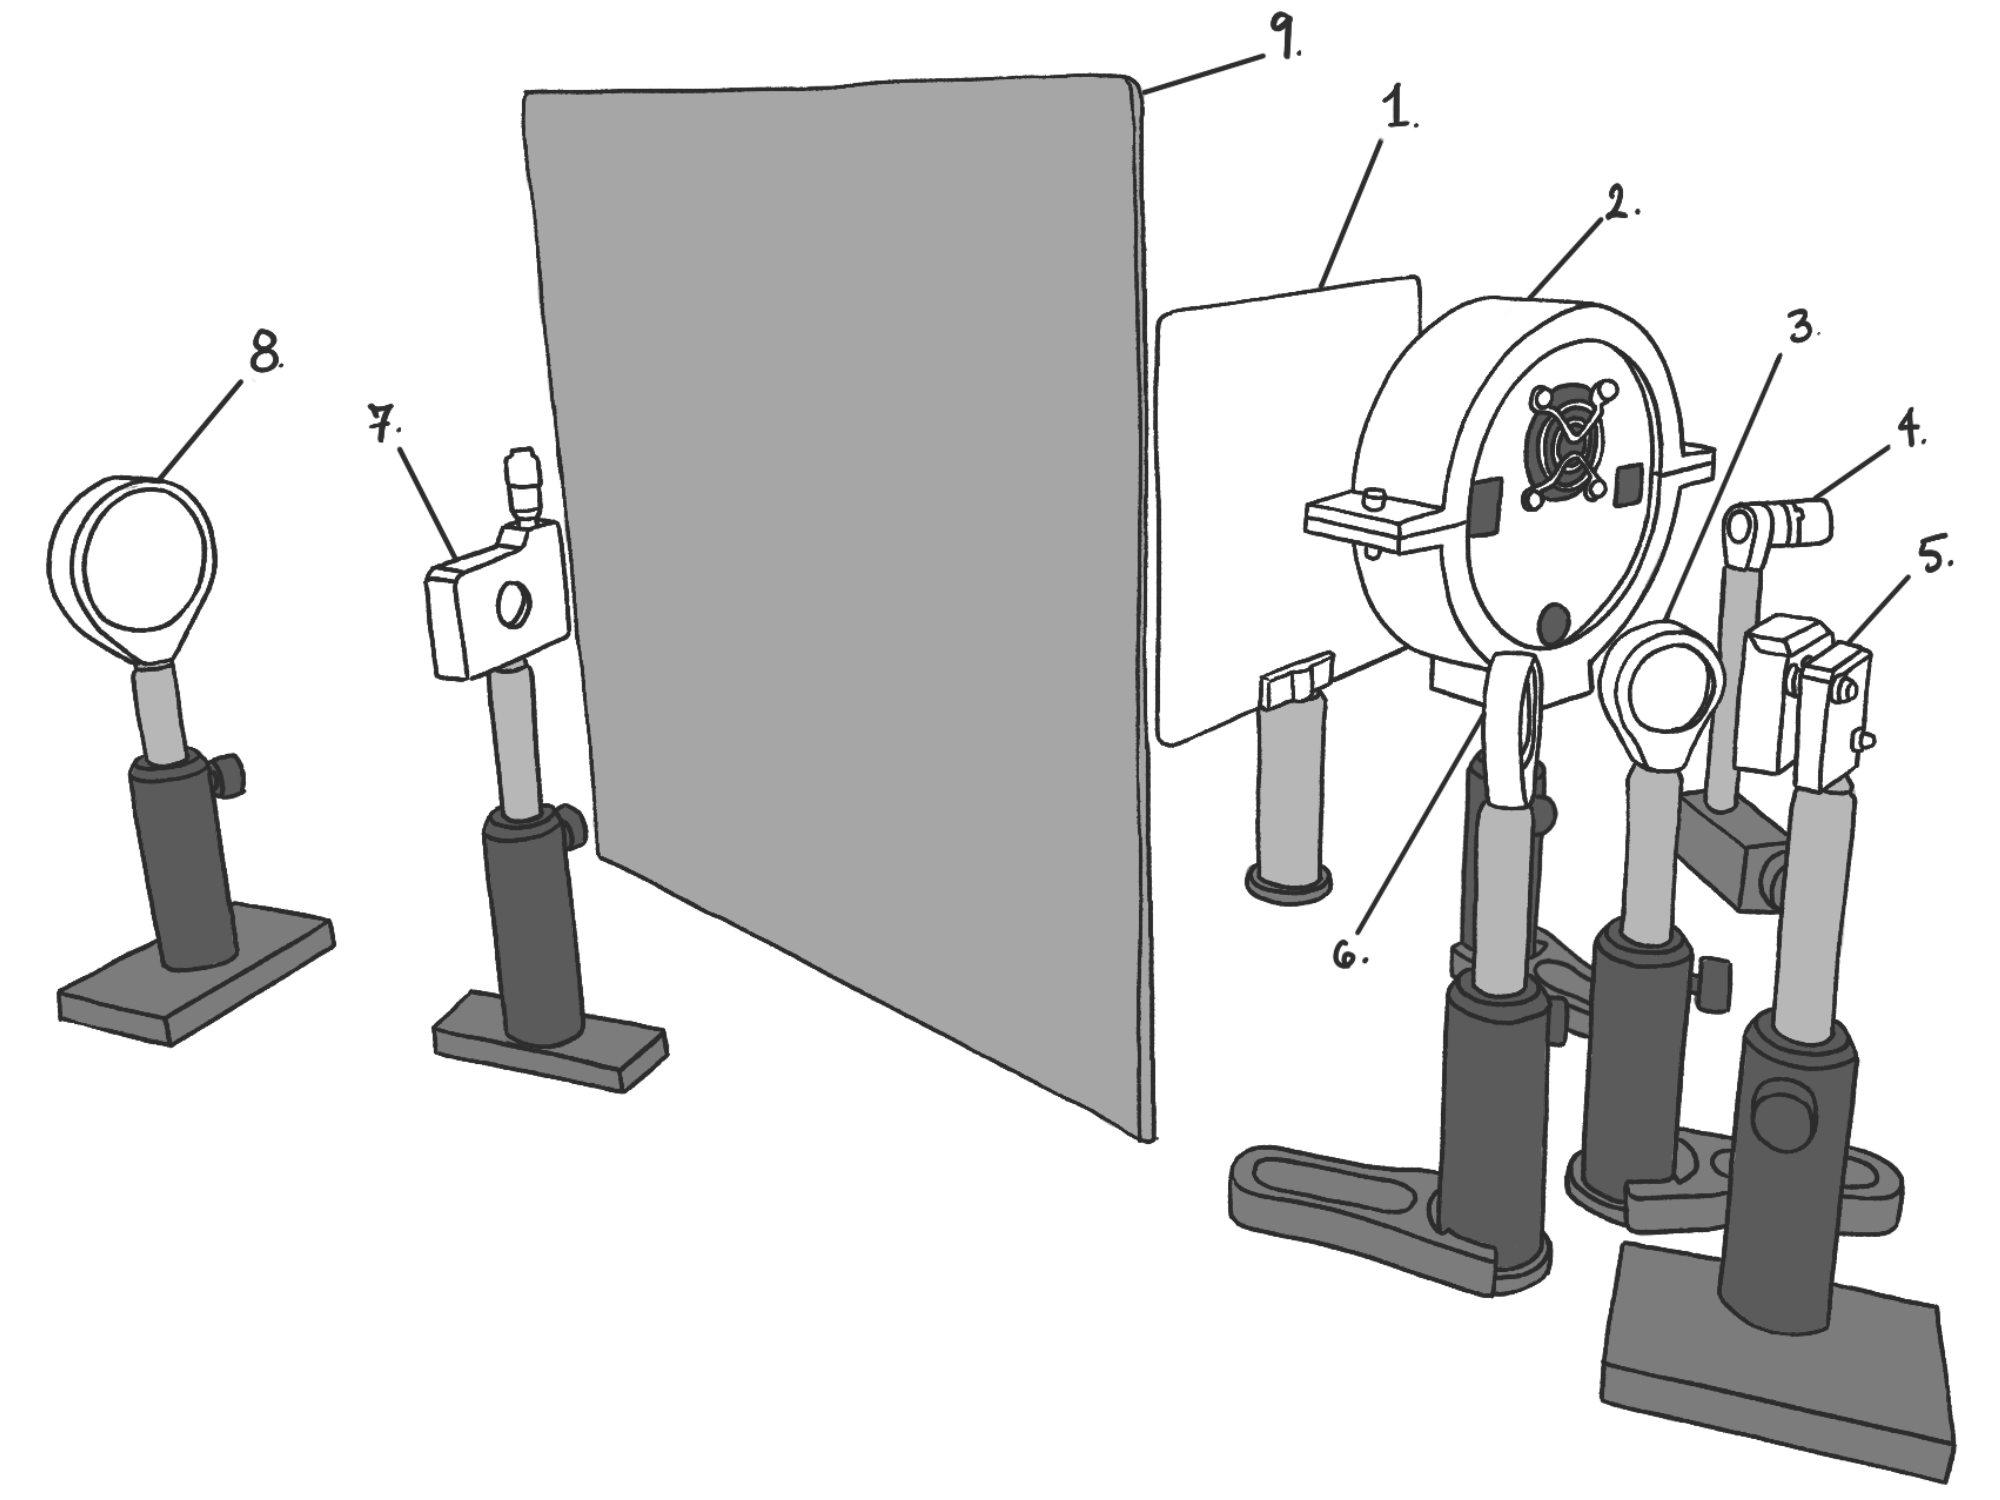
\includegraphics[width=\linewidth]{ccd_setup.PNG}
  \caption{CCD Spectrograph setup with: 1. screen, 2. CCD camera, 3. demagnifying lens, 4. LED, 5. diffraction grating, 6. collimator, 7. slit, 8. focusing lens, 9. blocking screen.}
  \label{fig:3}
\end{figure}

The LED (4) and screen (1) were used for the capture of the flat field and bias frames, while the mercury and sodium lamps (not shown) were used as the 
light sources for the spectral data acquisition. The lamps were positioned behind the focusing lens (8) in such a way that the light passed through all 
components of the spectrograph before reaching the CCD camera (2). The demagnifying lens (3) was used to reduce the size of the image projected onto the 
CCD, which were then visualised and captured using the \textit{Artemis Capture} software. The blocking screen (9) was used to prevent any light leakage
onto the CCD during image acquisition.

\subsection{Flats and Biases}

Since the CCD camera was cooled to at least -5°C using the built-in cooler, dark frames were not necessary for this lab. A series of 10 bias frames and
10 flat field frames were captured using an exposure time of 0.001 seconds. The flat fields were taken by illuminating the screen (1) with the LED (4) 
uniformly and ensuring that the CCD saturation level was not exceeded (less than 65536 counts) when viewed in the \textit{Artemis Capture} software. The
bias frames were taken with the shutter closed and same (near-zero) exposure time. The room was dark for all readings. Data collected was saved in FITS 
format for further analysis using a Python Jupyter notebook.

With 'master' bias and flat frames created by averaging the individual frames, the readout noise and gain of the CCD for corrections were calculated
using the following equations:

\begin{equation} \label{eq:1}
  \text{flatdif} = \text{flat}_1 - \text{flat}_2
\end{equation}

\begin{equation} \label{eq:2}
  \text{biasdif} = \text{bias}_1 - \text{bias}_2
\end{equation}

\begin{equation} \label{eq:3}
  \text{gain} = \frac{\left( \overline{\text{flat}_1} + \overline{\text{flat}_2} \right) - \left( \overline{\text{bias}_1} + \overline{\text{bias}_2} \right)}{\sigma^2_{\text{flatdif}} - \sigma^2_{\text{biasdif}}}
\end{equation}

\begin{equation} \label{eq:4}
  \text{readnoise} = \text{gain} \times \frac{\sigma_{\text{biasdif}}}{\sqrt{2}}
\end{equation}

Gain is the conversion factor from analog units (e$^-$)to digital units (ADU), while readout noise is the uncertainty in the number of electrons, caused
by the CCD electronics.

\subsection{Spectrograph Calibration}

By using the \textbf{mercury lamp} as the light source and taking a spectral image of the emitted light, the spectrograph was calibrated by comparing the known
emission lines to the pixel positions of the detected lines on the CCD. A clear image should be captured with well-defined, but not saturated, emission
lines. A calibration curve of the wavelength (nm) against the pixel position can be created, which can then be used to convert pixel positions in
subsequent spectral images to wavelengths using the same spectrograph setup.

\subsection{Spectrograph Resolution}

By using the \textbf{sodium lamp} as the light source and taking a spectral image of the emitted light, the spectral resolution of the spectrograph could 
be determined by measuring the full width at half maximum (FWHM) of a fitted Gaussian to the sodium D-lines in the obtained spectrum. The spectral 
resolution R is then given by:

\begin{equation} \label{eq:5}
  R = \lambda / \Delta \lambda
\end{equation}

with $\lambda$ as the wavelength converted with the calibration curve and $\Delta \lambda$ as the FWHM of the fitted Gaussian of the line. The resolution
indicates the ability of the spectrograph to distinguish between closely spaced spectral features. \cite{howell2000handbook}

\section{Results} \label{sec:3}

\subsection{Biases and Flats}

A series of bias images were taken with the CCD shutter closed, and a master bias frame was created by stacking and averaging the 
frames together, seen in Figure \ref{fig:4}.

\begin{figure}[H]
  \centering
  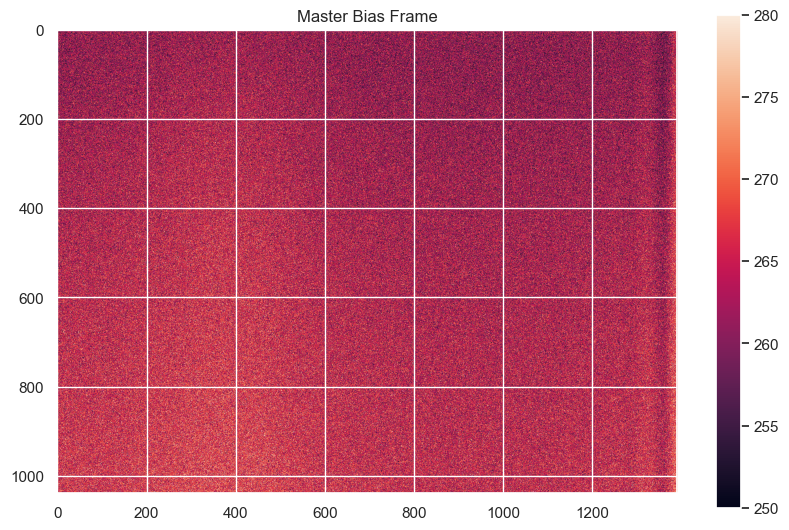
\includegraphics[width=.85\linewidth]{masterbias.png}
  \caption{Master bias frame}
  \label{fig:4}
\end{figure}

A series of flat images were taken of the CCD evenly illuminated by the LED and a master flat frame was created by stacking and 
averaging the frames together, subtracting the master bias frame from each individual flat frame beforehand, seen in Figure \ref{fig:5}.

\begin{figure}[H]
  \centering
  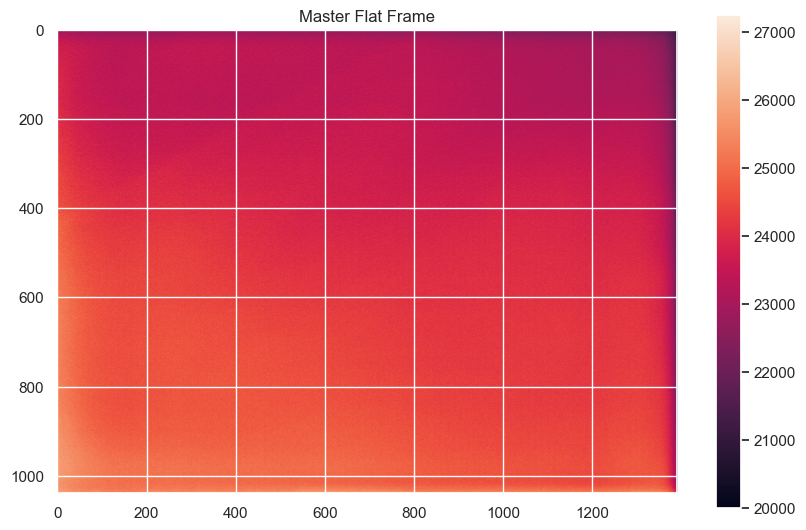
\includegraphics[width=.85\linewidth]{masterflat.png}
  \caption{Master Flat Frame}
  \label{fig:5}
\end{figure}

To calculate the average readnoise and gain of the CCD, equations \ref{eq:1}-\ref{eq:4} were applied to each image pair of the 10
bias and flat frames captured. The results for each image pair are summarised in Table \ref{tab:1}. From these individual values, the
average gain and readnoise were found to be \textbf{0.2700 e$^-$/ADU} and \textbf{4.4722 e$^-$} respectively. Referencing the CCD manual
\cite{atikseries3manual}, the typical readnoise is said to be 4 e$^-$. In the manual it is also stated that CCD has "less that 5
electrons RMS", so the obtained average readnoise falls within this performance range.

\begin{figure*}[ht]
  \centering
  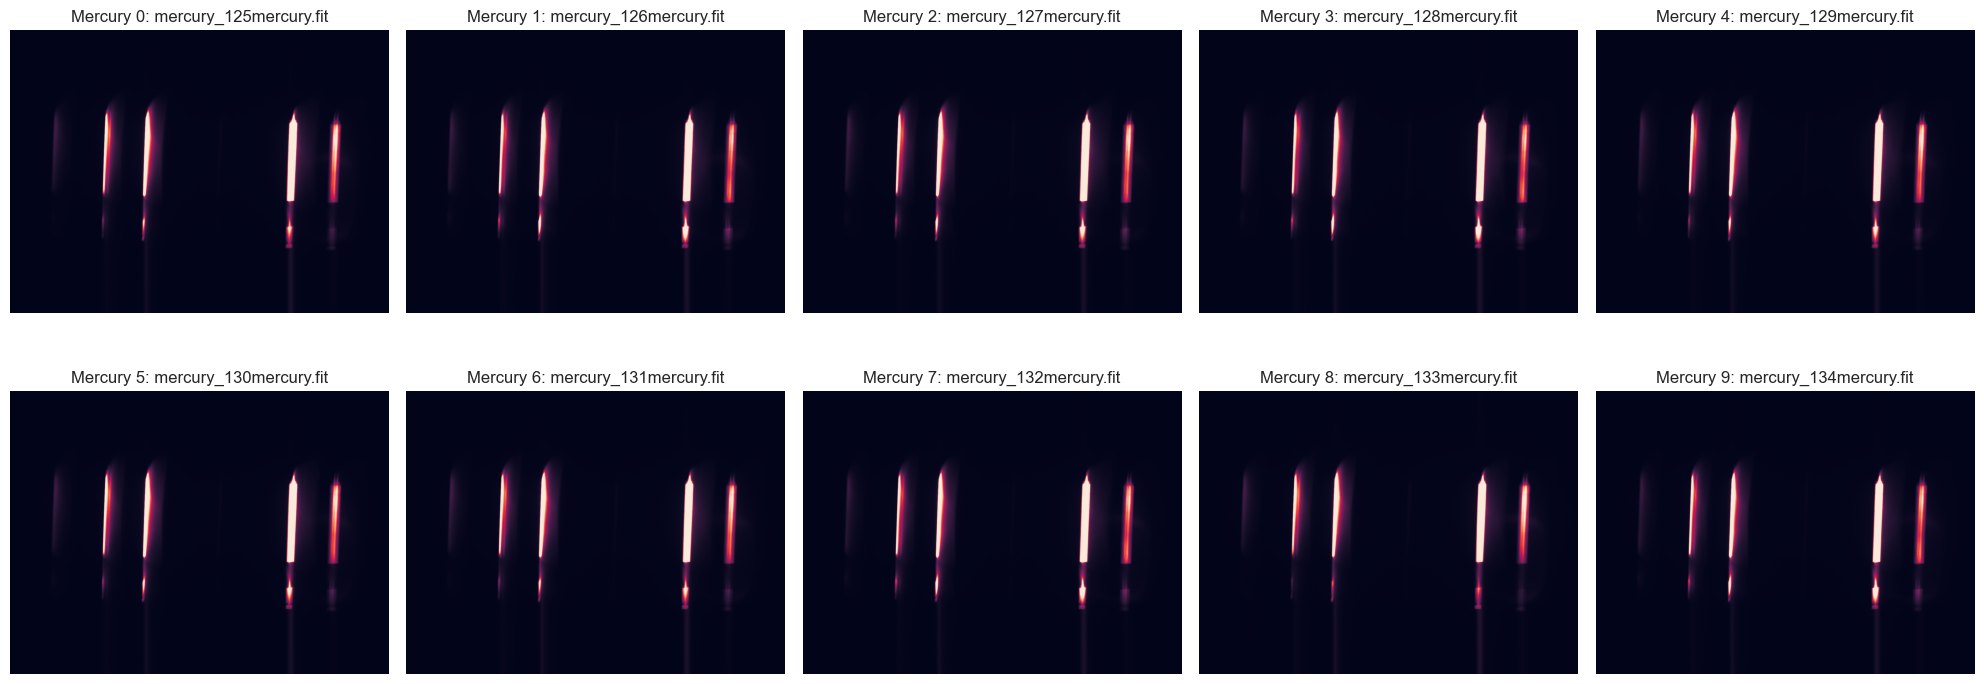
\includegraphics[width=\linewidth]{allmerc.png}
  \caption{10 Mercury spectral frames}
  \label{fig:6}
\end{figure*}

\subsection{Spectrograph Calibration}

\subsubsection{Mercury Spectrum}

By using the Mercury lamp in the CCD spectrograph configuration, 10 images of the resulting spectral lines were taken, see Fig. \ref{fig:6}.
Unfortunately, in order to display the far left spectral line the other lines were oversaturated (see Table \ref{tab:2}).
From these, one image was selected, seen in Fig. \ref{fig:7}.

\begin{figure}[H]
  \centering
  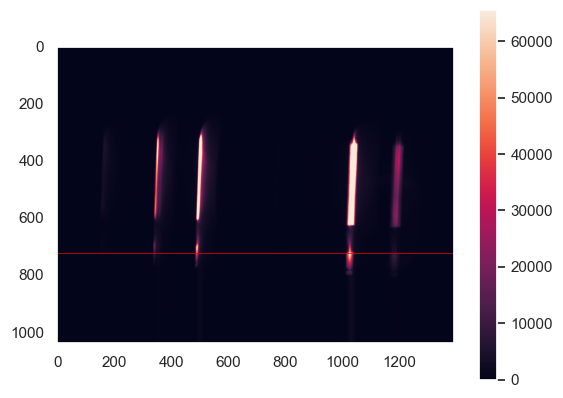
\includegraphics[width=.95\linewidth]{mercury.png}
  \caption{Mercury spectrum chosen from Fig. \ref{fig:6} (image 7) with indicated slice at y=725.}
  \label{fig:7}
\end{figure}

\begin{figure*}[hb]
  \centering
  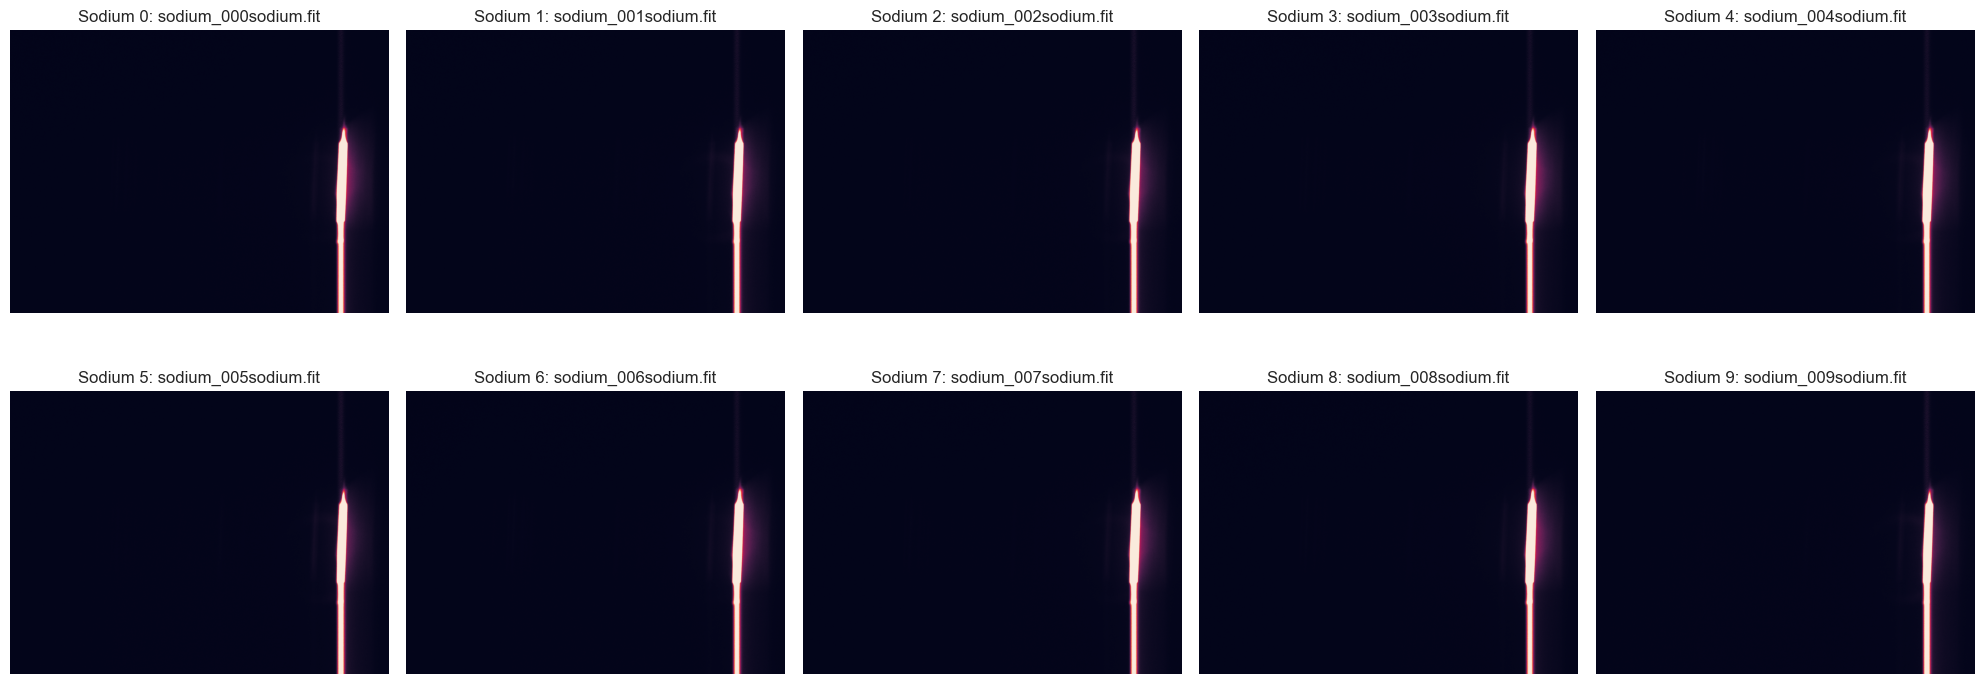
\includegraphics[width=\linewidth]{allsod.png}
  \caption{10 Sodium spectral frames}
  \label{fig:11}
\end{figure*}

\subsubsection{Calibration Curve} \label{sec:3.2.2}

By taking a slice of the spectral lines through y=725, all 5 peaks were retained without capping at maximum counts (see Fig. \ref{fig:8}).
Therefore, the peaks were well-defined and proper calculations for the calibration curve were made.

\begin{figure}[H]
  \centering
  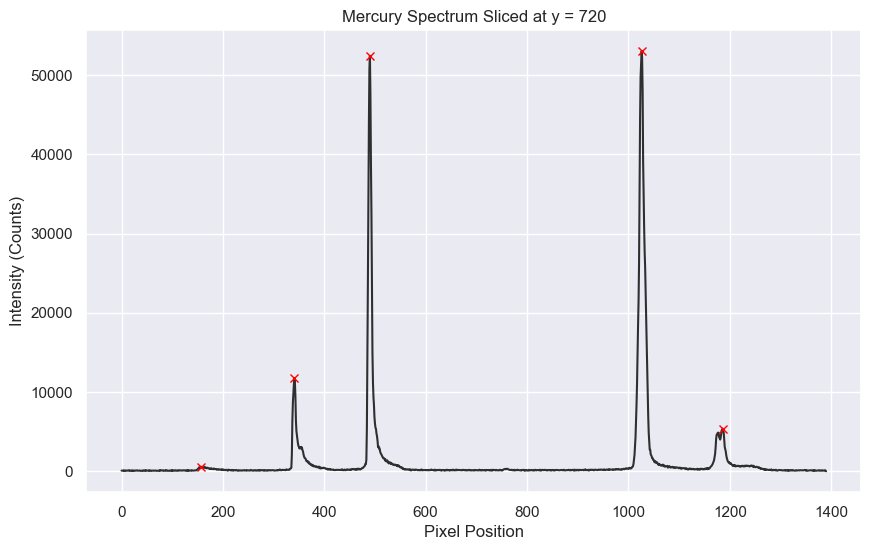
\includegraphics[width=.9\linewidth]{mercury_slice.png}
  \caption{Extracted mercury spectrum at y=725 with peaks indicated by red crosses.}
  \label{fig:8}
\end{figure}

Known emission lines of the Mercury spectrum were plotted against those captured by the spectrograph and labelled, seen in Fig. \ref{fig:9}.
The position of these peaks and intensities were summarised in Table \ref{tab:4}.

\begin{figure}[H]
  \centering
  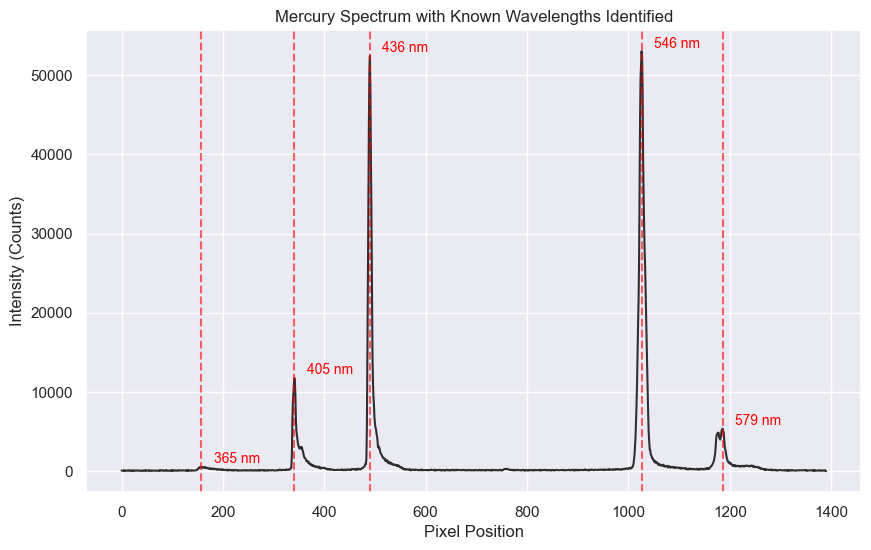
\includegraphics[width=.9\linewidth]{mercury_known.png}
  \caption{Extracted mercury spectrum at y=725 with known emission lines fitted and indicated by red dashed lines.}
  \label{fig:9}
\end{figure}

By using the x-position of the peaks and the known wavelengths of Mercury, a linear regression fit could be performed using
$y = mx + c$ and plotted, seen in Fig. \ref{fig:10}.

\begin{figure}[H]
  \centering
  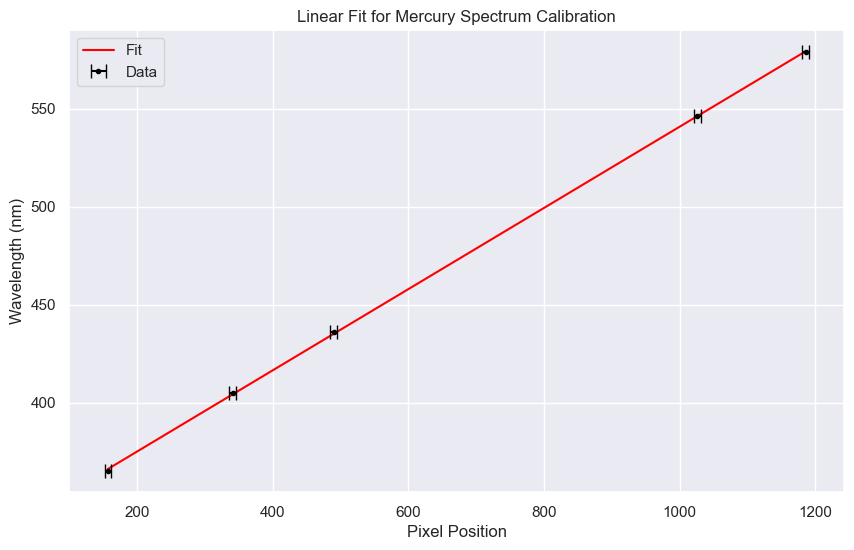
\includegraphics[width=.9\linewidth]{mercury_calibcurve.png}
  \caption{Calibration curve of wavelength (nm) against pixel position with linear fit.}
  \label{fig:10}
\end{figure}

The slope of the fit was found to be \textbf{0.2071 nm/px}, and the intercept to be \textbf{333.6445 nm}. These values could then be
used to convert the pixel positions on other spectral images to wavelenghts. By taking the residuals of the linear regression, which takes the error on
the actual data points to the fitted line ($e = y_{\text{actual}} - y_{\text{fit}}$), and then taking the standard deviation of the values the margin of
error of the Mercury calibration was found to be \textbf{0.7399 nm}.

\subsection{Spectrograph Resolution}

\subsubsection{Sodium Spectrum}

Switching the Mercury lamp for a Sodium lamp in the CCD spectrograph configuration, 10 images of the resulting spectral lines were taken, seen in Fig. \ref{fig:11}.
Summarised in Table \ref{tab:3}, the maximum and minimum counts for each image show that some images are oversaturated. Hence, one image was selected, seen
in Fig. \ref{fig:12}.

\begin{figure}[H]
  \centering
  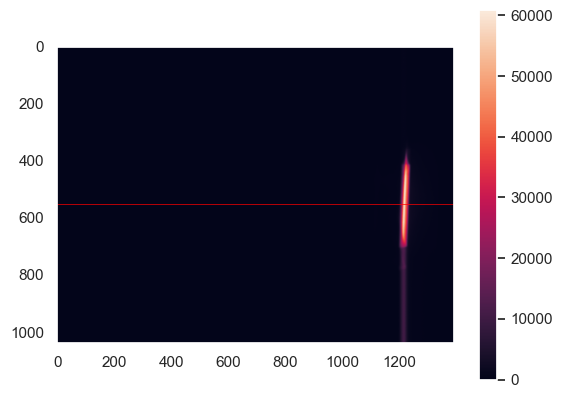
\includegraphics[width=.95\linewidth]{sodium.png}
  \caption{Sodium spectrum chosen from Fig. \ref{fig:11} (image 1) with indicated slice at y=550.}
  \label{fig:12}
\end{figure}

\subsubsection{Resolution Calculation}

By taking a slice of the spectral line at y=550, the peak position and intensity was plotted, seen in Fig. \ref{fig:13}. The peak position was found to be
1216 px with intensity of 58800.4.

\begin{figure}[H]
  \centering
  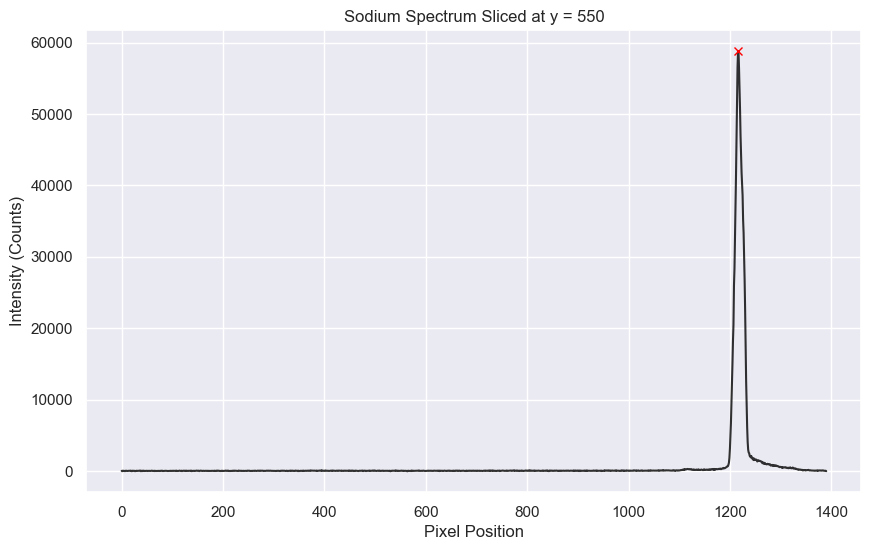
\includegraphics[width=.9\linewidth]{sodium_slice.png}
  \caption{Extracted sodium spectrum at y=550 with peak indicated by a red cross.}
  \label{fig:13}
\end{figure}

Using the calibration factors calculated in \hyperref[sec:3.2.2]{§3.2.2}, the spectral image of the Sodium lamp can be plotted against wavelength instead
of pixel positions. Zooming in on the peak and plotting the known D-lines for the Sodium spectrum, as seen in Fig. \ref{fig:14}, it can be seen that
the singular peak position does not align with the known values. The wavelength value of this peak, using the calibration curve, was found to be
\textbf{581.4781 nm}. The standard deviation of the obtained spectral line, using the median value of the D-lines as 589.3 nm, was determined as
\textbf{3.821 nm}, which is outside the Mercury calibration margin or error.

\begin{figure}[H]
  \centering
  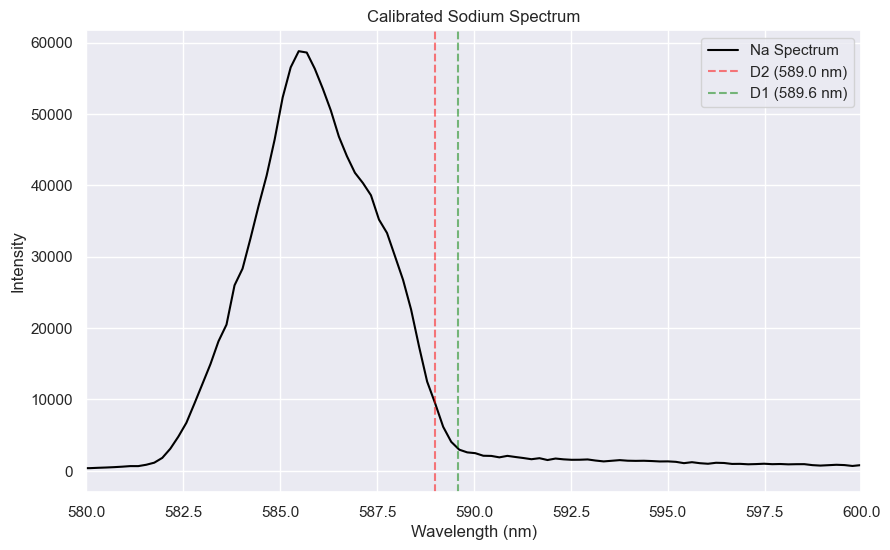
\includegraphics[width=.9\linewidth]{sodium_calibrated.png}
  \caption{Zoomed-in peak of extracted sodium spectrum at y=550 calibrated from results in \hyperref[sec:3.2.2]{§3.2.2} with known D-lines fitted and indicated by red dashed lines.}
  \label{fig:14}
\end{figure}

As can be seen by the values in Table \ref{tab:3}, and considering that images were taken with the minimum possible exposure time without oversaturating
the CCD, there were no two expected peaks that would represent the D-lines. However, when oversaturated, the spectrum shows another bright spectral line close
to the one found when not saturated, seen in Fig. \ref{fig:15}. However, due to the blooming of the oversaturated line, this image can not be used for
resolution calculations.

Instead, since Mercury agrees well with the known spectrum values and has well-defined peaks, to find the resolution of the spectrograph these were used.
Using a standard Gaussian with an offset (equation \ref{eq:6}) to fit to the individual curves, the resolution was found using equation \ref{eq:5}.

\begin{equation} \label{eq:6}
  f(x) = A e^{-\frac{(x - x_0)^2}{2 \sigma^2}} + \text{offset}
\end{equation}

with A as the amplitude (counts), x as the wavelength values (nm), x$_0$ as the peak's centre (nm), $\sigma$ as the width (nm), and the offset as the base
noise level.

While the Gaussians for each peak of the Mercury spectrum were not plotted, the values obtained and their errors are summarised in Table \ref{tab:5}. The 
full width at half maximum was converted with $\Delta \lambda = 2.335 \sigma$, with 2.335 as the conversion factor, and the resolution for the spectrograph
was then obtained with equation \ref{eq:5}.

For the 436 nm and 546 nm peaks, which are the most intense and well-defined peaks, the resolution was found to be \textbf{296.0 ±
11.3} and \textbf{221.0 ± 12.0} respectively. The errors for these values were calculated by the following formula:

\begin{equation}
  \delta R = R \sqrt{\left( \frac{\delta \lambda}{\lambda} \right) ^2 + \left( \frac{\delta \Delta \lambda}{\Delta \lambda} \right)^2}
\end{equation}

\section{Analysis and Discussion} \label{sec:4}

\subsection{CCD Characterisation}

The characterisation of the CCD camera using the bias and flat frames allowed for the determination of the gain and readnoise of
the CCD camera. The average gain was found to be \textbf{0.2700 e$^-$/ADU} and the average readnoise to be \textbf{4.4722 e$^-$}.
The value for the readnoise aligns closely manufacturer's specifications of approximately 4 e$^-$ and less than 5 e$^-$ RMS. \cite{atikseries3manual}

This consistency between the experimental and theoretical values indicates that the CCD camera was functioning within expected
parameters, providing confidence in the accuracy of the spectral images captured and that the master flat and bias frames effectively
corrected for pixel sensitivity variations and electronic offsets. The use of a cooled CCD minimised dark current contributions, thus 
dark frames were not necessary for the analysis. Errors could have arisen from fluctuations in temperature during image acquisition,
imperfections in the flat field illumination, or latency in the shutter mechanism during image capture.

\subsection{Spectrograph Calibration}

The spectograph setup was calibrated using the Mercury lamp and comparing the known emission lines to the pixel positions of the
CCD spectral image. A single image was selected from the 10 captured, and a slice at y=725 was taken to extract the spectrum, ensuring
all 5 key emission lines were present without clipping from saturation.

The calibration curve yielded a slope (dispersion) of \textbf{0.2071 nm/px} and an intercept of \textbf{333.646 nm}, so the
following relationship could be used to convert pixel positions to wavelengths:

\begin{equation*}
  \lambda = 0.2071 x + 333.646
\end{equation*}

The error in the calibration which is the standard deviation of the residuals from the linear fit was found to be \textbf{0.7399 nm},
which suggests that spectral lines separated by less than this value may not be correctly resolved and distinguished. Errors in the
calibration could have arisen from imprecise peak identification, minor misalignments in spectrograph components, and limitations 
from using a linear fit instead of a higher-order polynomial fit, such as a quadratic fit.

\subsection{Spectrograph Resolution}

To calculate and determine the spectrograph's resoltution, the Sodium lamp was used in place of the Mercury lamp. During analysis, it
was seen that the spectrograph was unable to resolve the two closely spaceed D-lines at 589.0 nm and 589.6 nm due to limitations in
the setup and CCD sensitivity, as despite using the minimum exposure time, some images had saturated pixels and only one peak was
visible. The extracted peak only showed a single peak at \textbf{581.4781 nm} instead of the expected doublet around a median value
of 589.3 nm. This standard deviation of this peak from the expected value was found to be \textbf{3.821 nm}, which is outside of the
Mercury calibration margin of error. This could suggest that the spectrograph alignment could have experience minor shifts between
readings or that the CCD sensitivity varied or was insufficient for the Sodium lamp intensity.

Due to being unable to extract meaningful resolution data from the Sodium lamp, the Mercury lamp data was used instead by fitting
Gaussians to the well-defined peaks in the spectrum. The strongest lines at 436 nm and 546 nm yielded resolutions of 
\textbf{296.0 ± 11.3} and \textbf{221.0 ± 12.0} respectively. The variations in resolution across the spectrum could be attributed
to wavelength-dependent factors, consistent with the broadening effects observed for the 579 nm peak for the Mercury lamp, which
had the largest uncertainties. This broadening could be due to reduced SNR at longer wavelengths, optical aberrations, or limitations
in the spectrograph setup.

\section{Conclusion}

This experiment successfully characterised a CCD camera and calibrated a spectrograph using known emission lines from a Mercury lamp.
The CCD characterisation yielded an average gain of \textbf{0.2700 e$^-$/ADU} and readnoise of \textbf{4.4722 e$^-$}. These values 
were found to align well within the manufacturer's specifications of "less than 5 RMS", confirming the CCD's proper functionality.

The spectrograph was calibrated with a Mercury lamp, resulting in a calibration curve defined by $y = 0.2071 x + 333.646$, which converts 
the pixel positions to wavelengths. The calibration margin of error was determined to be \textbf{0.7399 nm}, representing the
standard deviation of the residuals from the linear fit and the spectrograph's ability to resolve closely spaced spectral features.

Attempts to determine the spectrograph's resolution using a Sodium lamp were unsuccessful due to inability to resolve the closely
spaced D-line doublet, with a single peak observed at \textbf{581.4781 nm}. Instead, the resolving power R was calculated using the
Mercury lamp data. For the strongest lines at 436 nm and 546 nm, the resolutions were found to be \textbf{296.0 ± 11.3} and
\textbf{221.0 ± 12.0} respectively, demonstrating the spectrograph's ability to distinguish between spectral features separated
by a few nanometers.

Overall, the experiment successfully demonstrated the principles of CCD characterisations and calibration, as well as practical
spectrograph applications for analysis. While there were limitations in resolving the Sodium D-lines, the results obtained from the
Mercury lamp provided suitable insights into the spectrograph's performance and capabilities. Future improvements could involve
greater care when switching light sources to maintain alignment, exploring higher order polynomial fits for more precise calibration,
and using a more sensitive CCD or longer exposure times to better capture weaker spectral features.

%%%%%%%%%%%%%%%%%%%%

% References - switch to single column
\onecolumn

\bibliographystyle{IEEEtran}
\bibliography{PHYC30170References} \label{sec:ref}

\newpage

% Appendix - single column
\section*{Appendix} \label{sec:A}
\addcontentsline{toc}{section}{Appendix}

\subsection*{Tables}
\addcontentsline{toc}{subsection}{Tables}

\begin{table}[H]
  \centering
  \caption{Calculated gain and readnoise for each image pair for 10 images captured using equations \ref{eq:1}-\ref{eq:4}.}
\begin{tabular}{|
  >{\columncolor[HTML]{C0C0C0}}c |c|c|}
  \hline
  Image Pair Index & \cellcolor[HTML]{EFEFEF}Gain (e$^-$/ADU) & \cellcolor[HTML]{EFEFEF}Readnoise (e$^-$) \\ \hline
  1 \& 2           & 0.2696...                    & 4.4706...                         \\ \hline
  3 \& 4           & 0.2698...                    & 4.4717...                         \\ \hline
  5 \& 6           & 0.2699...                    & 4.4673...                         \\ \hline
  7 \& 8           & 0.2703...                    & 4.4791...                         \\ \hline
  9 \& 10          & 0.2701...                    & 4.4721...                         \\ \hline
\end{tabular}
\label{tab:1}
\end{table}

\begin{table}[H]
  \centering
  \begin{minipage}{.45\textwidth}
    \centering
    \caption{Maximum and minimum counts per spectral image for Mercury.}
    \vspace{1em}
    \label{tab:2}
    \resizebox{.99\textwidth}{!}{
    \begin{tabular}{|
    >{\columncolor[HTML]{C0C0C0}}c |c|c|}
    \hline
    Image Index & \cellcolor[HTML]{EFEFEF}Counts Min. & \cellcolor[HTML]{EFEFEF}Counts Max. \\ \hline
    0           & 217                                 & 65535                               \\ \hline
    1           & 215                                 & 65535                               \\ \hline
    2           & 214                                 & 65535                               \\ \hline
    3           & 215                                 & 65535                               \\ \hline
    4           & 216                                 & 65535                               \\ \hline
    5           & 208                                 & 65535                               \\ \hline
    6           & 217                                 & 65535                               \\ \hline
    7           & 0                                   & 65535                               \\ \hline
    8           & 218                                 & 65535                               \\ \hline
    9           & 211                                 & 65535                               \\ \hline
    \end{tabular}
    }
  \end{minipage}%
  \hfill%
  \begin{minipage}{.45\textwidth}
    \caption{Maximum and minimum counts per spectral image for Sodium.}
    \vspace{1em}
    \label{tab:3}
    \resizebox{.99\textwidth}{!}{
    \begin{tabular}{|
    >{\columncolor[HTML]{C0C0C0}}c |c|c|}
    \hline
    Image Index & \cellcolor[HTML]{EFEFEF}Counts Min. & \cellcolor[HTML]{EFEFEF}Counts Max. \\ \hline
    0           & 193                                 & 65535                               \\ \hline
    1           & 193                                 & 60921                               \\ \hline
    2           & 189                                 & 59868                               \\ \hline
    3           & 193                                 & 65535                               \\ \hline
    4           & 186                                 & 65535                               \\ \hline
    5           & 190                                 & 49077                               \\ \hline
    6           & 201                                 & 65535                               \\ \hline
    7           & 191                                 & 65535                               \\ \hline
    8           & 187                                 & 65535                               \\ \hline
    9           & 189                                 & 42236                               \\ \hline
    \end{tabular}
    }
  \end{minipage}
\end{table}

\begin{table}[H]
  \centering
  \caption{Peak x-positions (pixels) for the Mercury spectrum sliced at y=720 for Fig. \ref{fig:7}.}
  \vspace{1em}
  \label{tab:4}
  \begin{tabular}{|
  >{\columncolor[HTML]{C0C0C0}}c |c|c|}
  \hline
  Peak Index & \cellcolor[HTML]{EFEFEF}x-position (Pixels) & \cellcolor[HTML]{EFEFEF}Intensity (Counts) \\ \hline
  1          & 157                                         & 577.2                                      \\ \hline
  2          & 341                                         & 11767.5                                    \\ \hline
  3          & 490                                         & 52428.5                                    \\ \hline
  4          & 1026                                        & 53010.9                                    \\ \hline
  5          & 1186                                        & 5382.2                                     \\ \hline
  \end{tabular}
\end{table}

\begin{table}[H]
  \centering
  \caption{Fitted Gaussian values to the Mercury spectrum peaks to calculate FWHM ($\Delta \lambda$) and Resolution with fitting and calculation errors.}
  \vspace{1em}
  \label{tab:5}
  \resizebox{\textwidth}{!}{%
  \begin{tabular}{|
  >{\columncolor[HTML]{C0C0C0}}c |
  >{\columncolor[HTML]{C0C0C0}}c |
  >{\columncolor[HTML]{EFEFEF}}c |
  >{\columncolor[HTML]{EFEFEF}}c |c|c|}
  \hline
  Peak (Pixel) & Wavelength (nm) & Fitted Center (nm) & Fitted Width (nm) & \cellcolor[HTML]{EFEFEF}FWHM ($\Delta \lambda$) (nm) & \cellcolor[HTML]{EFEFEF}Resolution (R) \\ \hline
  341                   & 405                  & 404.2695 ± 0.0486  & 0.5909 ± 0.0562   & 1.391 ± 0.132                                        & 291.1 ± 27.7                           \\ \hline
  490                   & 436                  & 435.1193 ± 0.0204  & 0.6254 ± 0.0204   & 1.473 ± 0.056                                        & 296.0 ± 11.3                           \\ \hline
  1026                  & 546                  & 546.2202 ± 0.0339  & 1.0489 ± 0.0571   & 2.470 ± 0.135                                        & 221.0 ± 12.0                           \\ \hline
  1186                  & 579                  & 578.2830 ± 0.1012  & 2.1309 ± 0.4147   & 5.018 ± 0.977                                        & 115.4 ± 22.5                           \\ \hline
  \end{tabular}%
  }
\end{table}

\subsection*{Figures}
\addcontentsline{toc}{subsection}{Figures}

\begin{figure}[H]
  \centering
  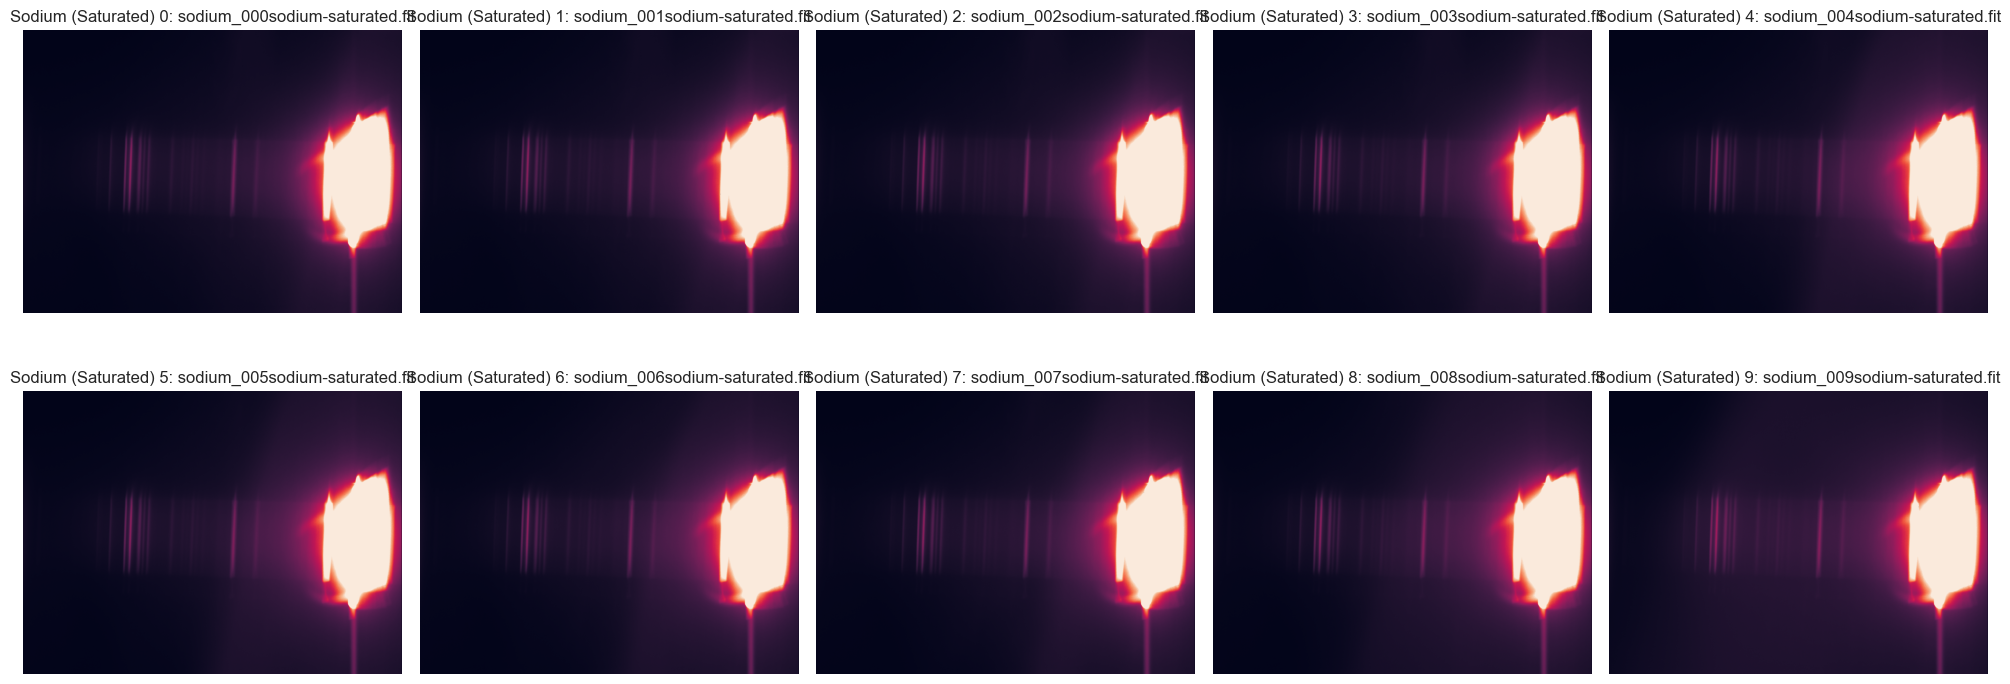
\includegraphics[width=\linewidth]{allsod_sat.png}
  \caption{Saturated images of the Sodium lamp spectrum.}
  \label{fig:15}
\end{figure}

\subsection*{Code}
\addcontentsline{toc}{subsection}{Code}

Can be found in the below pages.


\includepdf[pages={1-5,8-14,17-20,25-27}]{/Users/JoanaUCD/Library/CloudStorage/OneDrive-UniversityCollegeDublin/Labs/labs-files/tex Files/ccd_code.pdf}

\end{document}